\subsection{@Название подглавы 1@}

Это небольшая демонстрация настроенных окружений для теорем, доказательств и прочего.

\begin{thm}[Линейная зависимость двух векторов]{example_thm}
Два вектора $\mathbf{u}$ и $\mathbf{v}$ линейно зависимы тогда и только тогда, когда:
\begin{equation*}
    \exists \lambda \in \mathbb{R} \colon \mathbf{u} = \lambda \mathbf{v} \quad \text{или} \quad \mathbf{v} = \lambda \mathbf{u}.
\end{equation*}

\end{thm}

\begin{prf}[]{example_prf}
Необходимость: Если \( \mathbf{u} \) и \( \mathbf{v} \) линейно зависимы, то существуют коэффициенты $\alpha, \beta \in \mathbb{R}$, не равные нулю одновременно, такие что:
\begin{equation*}
    \alpha \mathbf{u} + \beta \mathbf{v} = \mathbf{0}.
\end{equation*}
Без ограничения общности, пусть \( \alpha \neq 0 \). Тогда:
\begin{equation*}
    \mathbf{u} = -\frac{\beta}{\alpha} \mathbf{v} = \lambda \mathbf{v}, \quad \text{где } \lambda = -\frac{\beta}{\alpha}.
\end{equation*}
Достаточность: Если $\mathbf{u} = \lambda \mathbf{v} $, то:
\begin{equation*}
    1 \cdot \mathbf{u} - \lambda \cdot \mathbf{v} = \mathbf{0},
\end{equation*}
что означает линейную зависимость $\mathbf{u}$ и $\mathbf{v}$ (коэффициенты $1$ и $-\lambda$ не равны нулю одновременно).
\end{prf}

\begin{lem}[О линейной зависимости]{example_lem}
    Если в наборе векторов $\mathbf{v}_1, \mathbf{v}_2, \dots, \mathbf{v}_k$ один из векторов является линейной комбинацией остальных, то этот набор линейно зависим.
\end{lem}

\newpage
\begin{dfn}[Собственные вектор и значение]{example_dfn}
Пусть $A$ - квадратная матрица размера $n \times n$.

\begin{itemize}
\item Ненулевой вектор $\mathbf{v} \in \mathbb{R}^n$ называется \textbf{собственным вектором} матрицы $A$, если существует число $\lambda \in \mathbb{R}$ такое, что:
$$ A\mathbf{v} = \lambda\mathbf{v} $$

\item Число $\lambda$ в этом случае называется \textbf{собственным значением} матрицы $A$, соответствующим вектору $\mathbf{v}$.
\end{itemize}

Эквивалентно, $\lambda$ является собственным значением, если:
\begin{equation*}
\det(A - \lambda I) = 0
\end{equation*}
где $I$ - единичная матрица соответствующего размера.
\end{dfn}{}

Вставка изображения:

\begin{figure}[h]
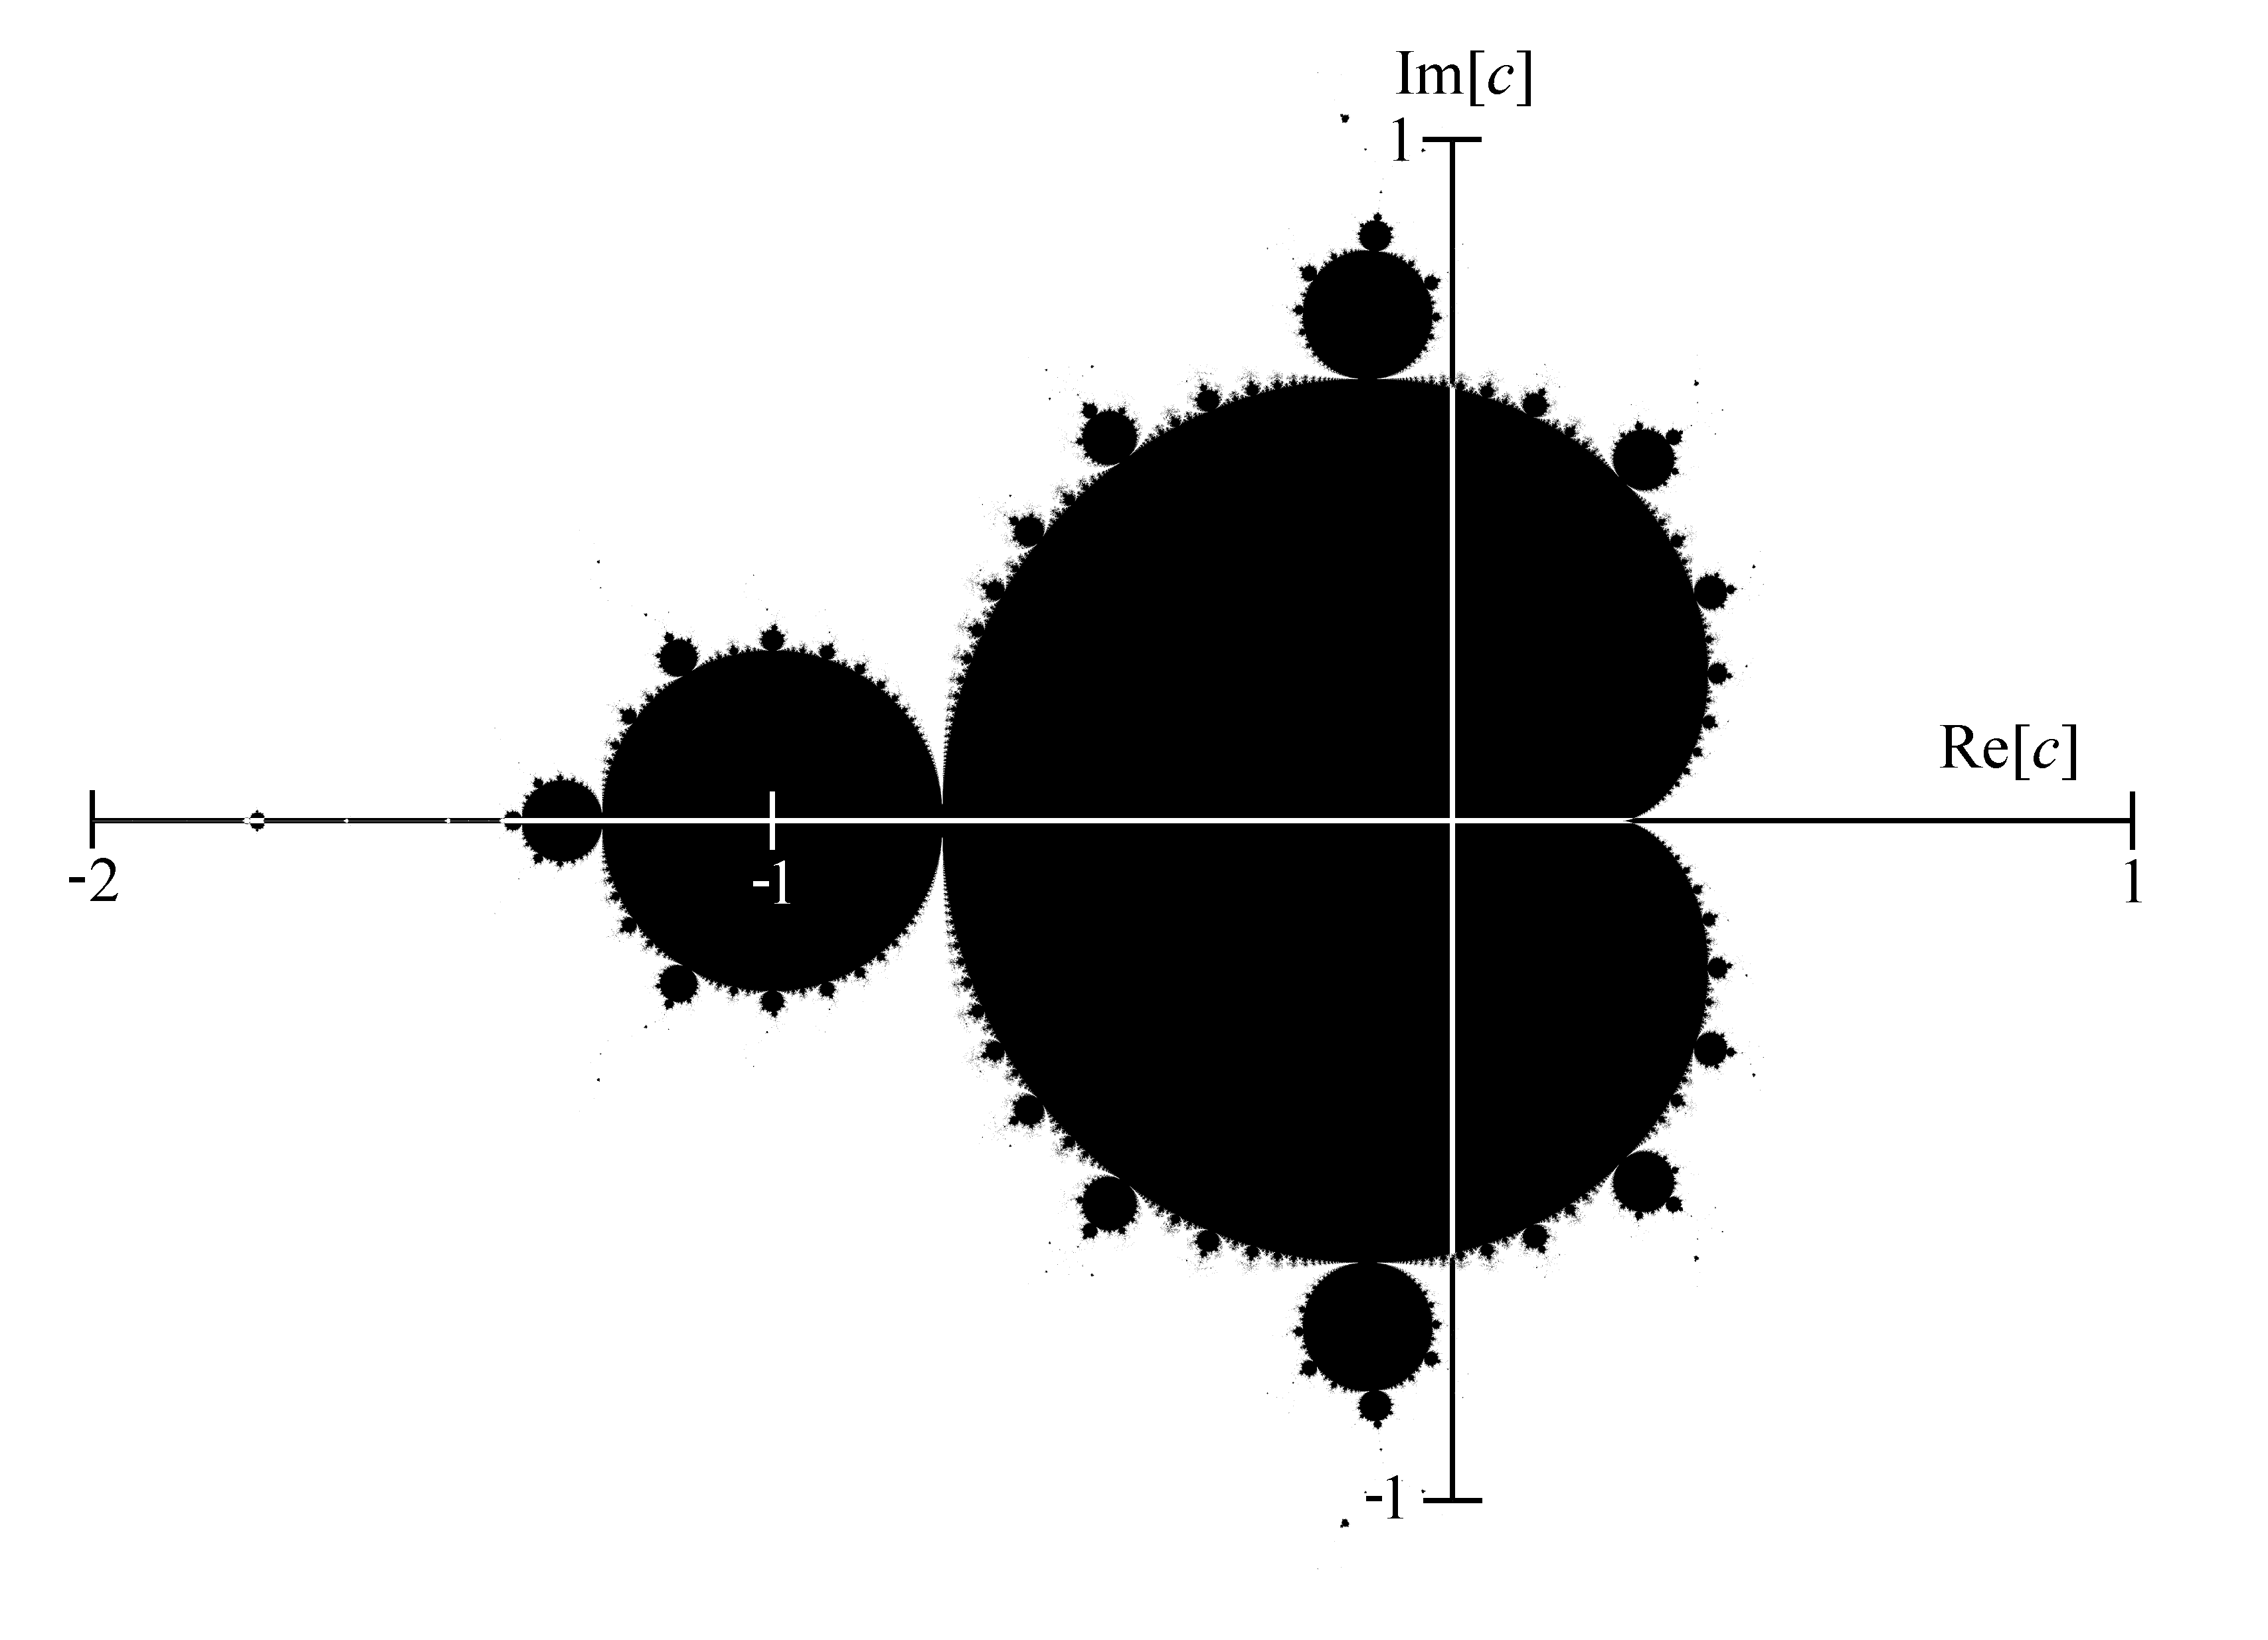
\includegraphics[width=15cm, angle=0]{mandelbrot_set.png}
\centering
\caption{Множество Мандельброта}
\end{figure}
